% This is samplepaper.tex, a sample chapter demonstrating the
% LLNCS macro package for Springer Computer Science proceedings;
% Version 2.20 of 2017/10/04
%
\documentclass[runningheads,table]{llncs}
%
\usepackage{graphicx}

% For algorithmic attachments and graphics
\usepackage{amsmath}
\usepackage{algorithm}
\usepackage[noend]{algpseudocode}
\usepackage{subcaption}
\captionsetup{compatibility=false}

\usepackage{tikz}
\usepackage{dsfont}
\usepackage{multicol, multirow}
\usepackage{textcomp}
%\usepackage{booktabs}
\usetikzlibrary{fit,calc,automata,positioning}


% Used for displaying a sample figure. If possible, figure files should
% be included in EPS format.
%
% If you use the hyperref package, please uncomment the following line
% to display URLs in blue roman font according to Springer's eBook style:
% \renewcommand\UrlFont{\color{blue}\rmfamily}

\begin{document}
%
\title{Context-Free Path Querying by Kronecker Product\thanks{The research was supported by the Russian Science Foundation, grant \textnumero 18-11-00100}}
%
%\titlerunning{Abbreviated paper title}
% If the paper title is too long for the running head, you can set
% an abbreviated paper title here
%
\author{Egor Orachev\inst{1} \and
Ilya Epelbaum\inst{1} \and
Rustam Azimov\inst{1,2} \and
Semyon~Grigorev\inst{1,2}\orcidID{0000-0002-7966-0698}}
%
\authorrunning{E. Orachev et al.}
% First names are abbreviated in the running head.
% If there are more than two authors, 'et al.' is used.
%
\institute{St.Petersburg State University, 7/9 Universitetskaya nab., St. Petersburg, Russia, 199034 \\
\email{egor.orachev@gmail.com, iliyepelbaun@gmail.com, rustam.azimov19021995@gmail.com, s.v.grigoriev@spbu.ru} \and
JetBrains Research, Primorskiy prospekt 68-70, Building 1, St. Petersburg, Russia, 197374\\
\email{semyon.grigorev@jetbrains.com}}
%
\maketitle              % typeset the header of the contribution
%
\begin{abstract}
Context-free path queries (CFPQ) extend the regular path queries (RPQ) by allowing context-free grammars to be used as constraints for paths.
Algorithms for CFPQ are actively developed, but J. Kuijpers et~al. have recently concluded, that existing algorithms are not performant enough to be used in real-world applications.
Thus the development of new algorithms for CFPQ is justified.
In this paper, we provide a new CFPQ algorithm which is based on such linear algebra operations as Kronecker product and transitive closure and handles grammars presented as recursive state machines.
Thus, the proposed algorithm can be implemented by using high-performance libraries and modern parallel hardware.
Moreover, it avoids grammar growth which provides the possibility for queries optimization.


\keywords{Context-free path querying \and Graph database \and Context-free grammars \and CFPQ \and Kronecker product \and Recursive state machines.}
\end{abstract}
%
%
%

\section{Introduction}


Language-constrained path querying~\cite{barrett2000formal} is a technique for graph navigation querying.
This technique allows one to use formal languages as constraints on paths in edge-labeled graphs: path satisfies constraints if labels along it form a word from the specified language.

The utilization of regular languages as constraints, or \textit{Regular Path Querying} (RPQ), is most well-studied and widespread.
Different aspects of RPQs are actively studied in graph databases~\cite{10.1145/2463664.2465216, 10.1145/3104031,10.1145/2850413}, while regular constraints are supported in such popular query languages as PGQL~\cite{10.1145/2960414.2960421} and SPARQL\footnote{Specification of regular constraints in SPARQL property paths: \url{https://www.w3.org/TR/sparql11-property-paths/}. Access date: 07.07.2020.}~\cite{10.1007/978-3-319-25007-6_1} (property paths).
Nevertheless, there is certainly room for improvement of RPQ efficiency, and new solutions are being created~\cite{Wang2019,10.1145/2949689.2949711}.

At the same time, using more powerful languages, namely context-free languages, as constraints has gained popularity in the last few years.
\textit{Context-Free Path Querying} problem (CFPQ) was introduced by Mihalis Yannakakis in 1990 in~\cite{Yannakakis}.
Many algorithms were proposed since that time, but recently, Jochem Kuijpers et al. showed in~\cite{Kuijpers:2019:ESC:3335783.3335791} that state-of-the-art CFPQ algorithms are not performant enough for practical use.
This motivates us to develop new algorithms for CFPQ.

One promising way to achieve high-performance solutions for graph analysis problems is to reduce them to linear algebra operations.
This way, GraphBLAS~\cite{7761646} API, the description of basic linear algebra primitives, was proposed.
Solutions that use libraries that implement this API, such as SuiteSparce~\cite{10.1145/3322125} and CombBLAS~\cite{10.1177/1094342011403516}, show that reduction to linear algebra is a way to utilize high-performance parallel and distributed computations for graph analysis.

Rustam Azimov shows in~\cite{Azimov:2018:CPQ:3210259.3210264} how to reduce CFPQ to matrix multiplication.
Later, it was shown in~\cite{Mishin:2019:ECP:3327964.3328503} and~\cite{10.1145/3398682.3399163} that utilization of appropriate libraries for linear algebra for Azimov's algorithm implementation makes a practical solution for CFPQ.
However Azimov's algorithm requires transforming the input grammar to Chomsky Normal Form, which leads to the grammar size increase, and hence worsens performance, especially for regular queries and complex context-free queries.

To solve these problems, an algorithm based on automata intersection was proposed~\cite{10.1007/978-3-030-54832-2_6}.
This algorithm is based on linear algebra and does not require the transformation of the input grammar.
We improve the algorithm in this work.
We reduce the above mentioned solution to operations over Boolean matrices, thus simplifying its description and implementation.
Also, we show that this algorithm is performant enough for regular queries, so it is a good candidate for integration with real-world query languages: one algorithm can be used to evaluate both regular and context-free queries.

Moreover, we show that this algorithm opens the way to tackle a long-standing problem about the existence of truly-subcubic $O(n^{3-\epsilon})$ CFPQ algorithm ~\cite{10.1145/1328438.1328460, Yannakakis}.
Currently, the best result is an $O(n^3/\log{n})$ algorithm of Swarat Chaudhuri~\cite{10.1145/1328438.1328460}.
Also, there exist truly subcubic solutions which use fast matrix multiplication for some fixed subclasses of context-free languages~\cite{8249039}.
Unfortunately, this solutions cannot be generalized to arbitrary CFPQs.
In this work, we identify incremental transitive closure as a bottleneck on the way to achieve subcubic time complexity for CFPQ.

To sum up, we make the following contributions.
\begin{enumerate}
	\item We rethink and improve the CFPQ algorithm based on tensor-product proposed by Orachev et al. ~\cite{10.1007/978-3-030-54832-2_6}.
	We reduce this algorithm to operations over Boolean matrices.
	As a result, all-path query semantics is handled, as opposed to the previous matrix-based solution which handles only the single-path semantics.
	Also, both regular and context-free grammars can be used as queries.
	We prove the correctness and time complexity for the proposed algorithm.
	\item We demonstrate the interconnection between CFPQ and incremental transitive closure.
	We show that incremental transitive closure is a bottleneck on the way to achieve faster CFPQ algorithm for general case of arbitrary graphs as well as for special families of graphs, such as planar graphs.
	\item We implement the described algorithm and evaluate it on real-world data for both RPQ and CFPQ. Results show that the proposed solution is comparable with existing solutions for CFPQ and RPQ, thus it is a promising way to create a unified algorithm for both CFPQ and RPQ evaluation.
\end{enumerate}
\section{Recursive State Machines}
\label{section:rsm}

In this section, we introduce recursive state machines (RSM)~\cite{rsm:analysis:10.1007/3-540-44585-4_18}.
This kind of computational machine extends the definition of finite state machines and increases the computational capabilities of this formalism.

A recursive state machine $R$ over a finite alphabet $\Sigma$ is defined as a tuple of elements $(M,m,\{C_i\}_{i \in M})$, where:

\begin{itemize}
    \item $M$ is a finite set of labels of boxes.
    \item $m \in M$ is an initial box label.
    \item Set of \textit{component state machines} or \textit{boxes},
          where $C_i=(\Sigma \cup M, Q_i,q_i^0,F_i,\delta_i)$:
    \begin{itemize}
        \item $\Sigma \cup M$ is a set of symbols, $\Sigma \cap M = \emptyset$
        \item $Q_i$ is a finite set of states,
              where $Q_i \cap Q_j = \emptyset, \forall i \neq j$
        \item $q_i^0$ is an initial state for the component state machine $C_i$
        \item $F_i$ is a set of final states for $C_i$, where $F_i \subseteq Q_i$
        \item $\delta_i$ is a transition function for $C_i$,
              where $\delta_i: Q_i \times (\Sigma \cup M)
              \to Q_i$
    \end{itemize}
\end{itemize}

RSM behaves as a set of finite state machines (or FSM).
Each FSM is called a \textit{box} or a \textit{component state machine}~\cite{rsm:analysis:10.1007/3-540-44585-4_18}.
A box works almost the same as a classical FSM, but it also handles additional \textit{recursive calls} and employs an implicit \textit{call stack} to \textit{call} one component from another and then return execution flow back.

The execution of an RSM could be defined as a sequence of the configuration transitions, which are done on input symbols reading. 
The pair $(q_i,S)$, where $q_i$ is current state for box $C_i$ and $S$ is stack of \textit{return states}, describes execution configurations. 

The RSM execution starts form configuration $(q_m^0, \langle\rangle)$. 
The following list of rules defines the machine transition from configuration $(q_i,S)$ to $(q',S')$ on some input symbol $a$ from the input sequence, which is read as usual for FSA:

\begin{itemize}
    \item $q' \gets q_i^t, S' \gets S$, where $q_i^t = \delta_i (q_i^k, a), q_i^k = q$
    \item $q' \gets q_j^0, S' \gets q_i^t \circ S$, where $q_i^t = \delta_i (q_i^k, j),  q_i^k = q, j \in M$
    \item $q' \gets q_i^t, S' \gets S_{tail}$, where $S = q_i^t \circ S_{tail}, q_j^k = q, q_j^k \in F_j$
\end{itemize}

Some input sequence of the symbols $a_1 ... a_n$, which forms some input word, accepted, if machine reaches configuration $(q,\langle\rangle)$, where $q \in F_m$. It is also worth noting that the  RSM makes not deterministic transitions, without reading the input character when it \textit{calls} some component or makes a \textit{return}.

%The execution of RSM $R$ is a sequance of transitions between configurations of form $(q,S)$, where $S$ is global stack of \textit{return states} from $\bigcup_{i \in M}Q_i$ such as $S=\langle ...q_r \rangle$, and $q \in \bigcup_{i \in M}Q_i$ is a current state of the machine. The execution starts from box $m$ initial state $q_m^0$ and empty stack as follows $(q_m^0,\langle \rangle)$. Transitions for a given global machine state $(q,S)$ to some new state $(q',S')$ are defined as follows:

%\begin{itemize}
%    \item $q':=q_b', S':=S$,
%    where $\delta_b (q_b,s) \to q_b', s \in \Sigma,
%    q=q_b, S = \langle ...q_r \rangle$
%    \item $q':=q_t^0, S':=\langle ...q_r,q_b'\rangle$,
%    where $\delta_b (q_b,t) \to q_b', t \in M, q=q_b, S = \langle ...q_r \rangle$
%    \item $q':=q_b', S':=\langle ...q_r \rangle$,
%    where $q=q_t^i, q_t^i \in F_t, S=\langle ...q_r,q_b' \rangle$
%\end{itemize}

According to~\cite{rsm:analysis:10.1007/3-540-44585-4_18}, recursive state machines are equivalent to pushdown systems.
Since pushdown systems are capable of accepting context-free languages~\cite{automata:theory:10.5555/1177300}, it is clear that RSMs are equivalent to context-free languages.
Thus RSMs suit to encode query grammars.
Any CFG can be easily converted to an RSM with one box per nonterminal.
The box which corresponds to a nonterminal $A$ is constructed using the right-hand side of each rule for $A$.
An example of such RSM $R$ constructed for the grammar $G$ with rules $S \to a S b \mid a b$ is provided in figure~\ref{example:automata}.

%We escape detailed discussion of the conversion of a context free grammar $G$ to a RSM $R$. In the basic case, an algorithm for constructing such RSM could be composed from several stages, where each stage involves building of finite state machine for each non-terminal $N$ from grammar $G$.

Since $R$ is a set of FSMs, it is useful to represent $R$ as an adjacency matrix for the graph where vertices are states from $\bigcup_{i \in M}Q_i$ and edges are transitions between $q_i^a$ and $q_i^b$ with label $l \in \Sigma \cup M$, if $\delta_i (q_i^a, l) = q_i^b$.
An example of such adjacency matrix $M_R$ for the machine $R$ is provided in section~\ref{example:section}.

\begin{figure}[h]
    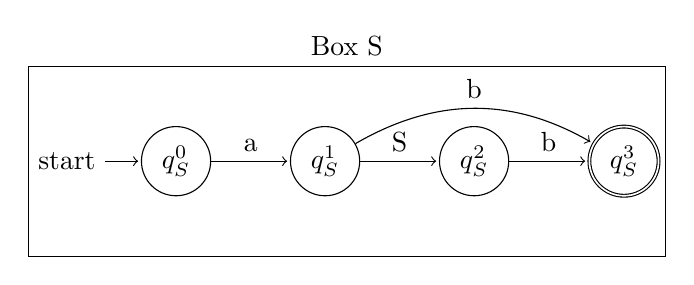
\begin{tikzpicture}[shorten >=1pt,auto]
        \node[state, initial] (q_0)   {$q_S^0$};
        \node[state] (q_1) [right=of q_0] {$q_S^1$};
        \node[state] (q_2) [right=of q_1] {$q_S^2$};
        \node[state, accepting] (q_3) [right=of q_2] {$q_S^3$};
        \path[->]
            (q_0) edge node {a} (q_1)
            (q_1) edge node {S} (q_2)
            (q_2) edge node {b} (q_3)
            (q_1) edge [bend left, above]  node {b} (q_3);
        \node[draw=black, fit= (q_0) (q_1) (q_2) (q_3), xshift=-4.5ex,inner sep=0.75cm, label=Box S] {};
    \end{tikzpicture}
    \centering
    \caption{The recursive state machine $R$ for grammar $G$}
    \label{example:automata}
\end{figure}


\section{Kronecker Product}
\label{kronecker:section}

In this section, we introduce the Kronecker product definition and its relation to the RSM and a directed graph intersection.

A directed labeled graph could be interpreted as an FSM, where transitions correspond to the labeled edges between vertices of the graph. 
As initial and final states could be chosen all vertices of the graph since this formal decision does not affect the algorithm idea.
As shown in the section~\ref{section:rsm}, an RSM is composed of a set of component state machines, which behave as a normal FSM. 
Notice, that these component machines are structurally independent, and actual communications are done only on \textit{recursive calls} in time of the machine execution. 
It makes an intuition that one could apply automata theory to intersect an RSM with a directed graph.

The classical intersection algorithm of two deterministic FSMs is presented in~\cite{automata:theory:10.5555/1177300}. 
The idea behind this algorithm is to create new FSM, which imitates the parallel work of both machines through an increase in the number of states and transitions. 
For any given FSMs $C_1 = (\Sigma \cup M,Q_1,q_1^0,F_1,\delta_1)$ and $C_2 = (\Sigma \cup M,Q_2,q_2^0,F_2,\delta_2)$ the intersection machine $C$ defines as follows: 

$C = (\Sigma \cup M, Q, q^0, F, \delta)$, where:

\begin{itemize}
    \item States $Q = \{(q_1,q_2)~:~q_1 \in Q_1, q_2 \in Q_2 \}$
    \item Final states $F = \{(q_1,q_2)~:~q_1 \in F_1, q_2 \in F_2 \}$
    \item Initial state $q = (q_1^0,q_2^0)$
    \item Transition function $\delta ((q_1,q_2),a) \to (\delta_1(q_1,a),\delta_2(q_2,a))$, where $a \in \Sigma \cup M$, only if $(\delta_1(q_1,a)$ and $\delta_2(q_2,a)$ are present.
\end{itemize}

A structurally similar procedure for constructing an intersection machine can be implemented using the Kronecker product for the corresponding transition matrices for FSMs if we provide a satisfying operation of elementwise multiplication, which allows further use of high-performance math libraries for intersection computation.

Since an RSM transitions matrix is composed as a blocked matrix of component state machines adjacency matrices, and a directed labeled graph could be presented as an adjacency matrix, it is convenient to implement the intersection of such objects via Kronecker product of the corresponding matrices. As an elementwise operation for one can employ the following function $\bullet: \Sigma \cup M \times \Sigma \cup M \to Boolean$, defined as follows: 

\begin{itemize}
    \item $A_1 \bullet A_2 = true$, if $A_1 \cap A_2 \neq \O$
    \item $A_1 \bullet A_2 = false$, otherwise
\end{itemize}

An example of applying the Kronecker product is illustrated in the section~\ref{example:section}. 

The operation defined in this way allows us to construct an adjacency Boolean matrix for some directed graph, where a path between two vertices exists only if corresponding paths exist in some component state machine of the RSM and in source graph at the same time. 
This fact with transitive closure could be employed in order to extract all the path and components labels from $M$ for context-free reachability problem-solving.
\section{Kronecker Product Based CFPQ Algorithm}

In this section, we introduce the algorithm for the computation of context-free reachability in a graph $\mathcal{G}$.
The algorithm determines the existence of a path, which forms a sentence of the language defined by the input RSM $R$, between each pair of vertices in the graph $\mathcal{G}$.
The algorithm is based on the generalization of the FSM intersection for an RSM, and an input graph. The idea of using the Kronecker product for the intersection of an RSM and a directed input graph is presented in the section~\ref{kronecker:section}.

% Since a graph can be interpreted as a FSM, in which transitions correspond to the labeled edges between vertices of the graph, and an RSM is composed of a set of FSMs, the intersection of such machines can be computed using the classical algorithm for FSM intersection, presented in~\cite{automata:theory:10.5555/1177300}.

% The intersection can be computed as a Kronecker product of the corresponding adjacency matrices for an RSM and a graph.
% Since we are only determining the reachability of vertices, it is enough to represent intersection result as a Boolean matrix.
% It simplifies the algorithm implementation and allows one to express it in terms of basic matrix operations.

Listing~\ref{tensor:cfpq} shows the main steps of the algorithm.
The algorithm accepts context-free grammar $G=(\Sigma,N,P$) and graph $\mathcal{G}=(V,E,L)$ as an input.
An RSM $R$ is created from the grammar $G$.
Note, that $R$ must have no $\varepsilon$-transitions.
$M_1$ and $M_2$ are the adjacency matrices for the machine $R$ and the graph $\mathcal{G}$ correspondingly.

Then for each vertex $i$ of the graph $\mathcal{G}$, the algorithm adds loops with non-terminals, which allows deriving $\varepsilon$-word.
Here the following rule is implied: each vertex of the graph is reachable by itself through an $\varepsilon$-transition.
Since the machine $R$ does not have any $\varepsilon$-transitions, the $\varepsilon$-word could be derived only if a state $s$ in the box $B$ of the $R$ is both initial and final.
This data is queried by the $getNonterminals()$ function for each state $s$.

The algorithm terminates when the matrix $M_2$ stops changing.
Kronecker product of matrices $M_1$ and $M_2$ is evaluated for each iteration.
The result is stored in $M_3$ as a Boolean matrix.
For the given $M_3$ a $C_3$ matrix is evaluated by the $transitiveClosure()$ function call.
The $M_3$ could be interpreted as an adjacency matrix for a directed graph with no labels, used to evaluate transitive closure in terms of classical graph definition of this operation.
Then the algorithm iterates over cells of the $C_3$.
For the pair of indices $(i,j)$, it computes $s$ and $f$ --- the initial and final states in the recursive automata $R$ which relate to the concrete $C_3[i,j]$ of the closure matrix.
If the given $s$ and $f$ belong to the same box $B$ of $R$, $s = q_B^0$, and $f \in F_B$, then $getNonterminals()$ returns the respective non-terminal.
If the condition holds then the algorithm adds the computed non-terminals to the respective cell of the adjacency matrix $M_2$ of the graph.

The functions $getStates$ and $getCoordinates$ (see listing~\ref{tensor:cfpq:help}) are used to map indices between Kronecker product arguments and the result matrix.
The Implementation appeals to the blocked structure of the matrix $C_3$, where each block corresponds to some automata and graph edge.

The algorithm returns the updated matrix $M_2$ which contains the initial graph $\mathcal{G}$ data as well as non-terminals from $N$.
If a cell $M_2[i,j]$ for any valid indices $i$ and $j$ contains symbol $S \in N$, then vertex $j$ is reachable from vertex $i$ in grammar $G$ for non-terminal $S$.


\begin{algorithm}[h]
\floatname{algorithm}{Listing}
\begin{algorithmic}[1]
\caption{Kronecker product based CFPQ}
\label{tensor:cfpq}
\Function{contextFreePathQuerying}{G, $\mathcal{G}$}
    % Input data preparation
    \State{$R \gets$ Recursive automata for $G$}
    \State{$M_1 \gets$ Adjacency matrix for $R$}
    \State{$M_2 \gets$ Adjacency matrix for $\mathcal{G}$}
    % Eps-transition handling for graph
    \For{$s \in 0..dim(M_1)-1$}
        \For{$i \in 0..dim(M_2)-1$}
            \State{$M_2[i,i] \gets M_2[i,i] \cup \textit{getNonterminals}(R,s,s)$}
        \EndFor
    \EndFor
    \While{Matrix $M_2$ is changing}
        \State{$M_3 \gets M_1 \otimes M_2$}
        \Comment{Evaluate Kronecker product}
        \State{$C_3 \gets \textit{transitiveClosure}(M_3)$}
        \State{$n \gets$ dim($M_3)$}
        \Comment{Matrix $M_3$ size = $n \times n$}
        % Add non-terminals (possibly new)
        \For{$i \in 0..n-1$}
           \For{$j \in 0..n-1$}
                \If{$C_3[i,j]$}
                    \State{$s, f \gets \textit{getStates}(C_3,i,j)$}
                    \If{$\textit{getNonterminals}(R,s,f) \neq \emptyset$}
                        \State{$x, y \gets \textit{getCoordinates}(C_3,i,j)$}
                        \State{$M_2[x,y] \gets M_2[x,y] \cup \textit{getNonterminals}(R,s,f)$}
                    \EndIf
                \EndIf
           \EndFor
        \EndFor
    \EndWhile
\State \Return $M_2$
\EndFunction
\end{algorithmic}
\end{algorithm}

\begin{algorithm}[h]
\floatname{algorithm}{Listing}
\begin{algorithmic}[1]
\caption{Help functions for Kronecker product based CFPQ}
\label{tensor:cfpq:help}
\Function{getStates}{$C, i, j$}
    \State{$r \gets dim(M_1)$}
    \Comment{$M_1$ is adjacency matrix for automata $R$}
    \State \Return{$\left\lfloor{i / r}\right\rfloor, \left\lfloor{j / r}\right\rfloor$}
\EndFunction
\Function{getCoordinates}{$C, i, j$}
    \State{$n \gets dim(M_2)$}
    \Comment{$M_2$ is adjacency matrix for graph $\mathcal{G}$}
    \State \Return{$i \bmod n, j \bmod n$}
\EndFunction
\end{algorithmic}
\end{algorithm}

\subsection{Example}
\label{example:section}

This section provides a step-by-step demonstration of the presented algorithm.
We consider the theoretical worst case for CFPQ time complexity, proposed by J.Hellings~\cite{hellings2015querying} as an example: the graph $\mathcal{G}$ is presented in Figure~\ref{input:graph} and the context-free grammar $G$ for a language $\{a^n b^n~|~n \geq 1\}$ is $ S \to a S b \mid a b$.

Since the proposed algorithm processes grammar in the form of a recursive machine, we first provide RSM $R$ in Figure~\ref{example:automata}.
The initial box of the $R$ is $S$, the initial state $q_S^0$ is $(0)$, the set of final states $F_S = \{ (3) \}$.

\begin{figure}[h]
        \centering
        \begin{subfigure}{.48\textwidth}
        \begin{center}
        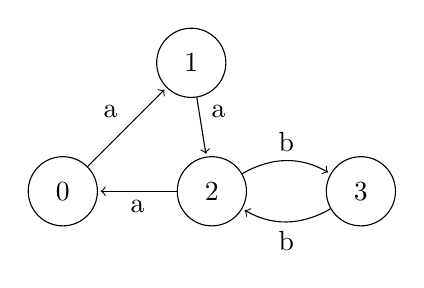
\begin{tikzpicture}[shorten >=1pt,auto]
           \node[state] (q_0)                      {$0$};
           \node[state] (q_1) [above right=of q_0] {$1$};
           \node[state] (q_2) [right=of q_0]       {$2$};
           \node[state] (q_3) [right=of q_2]       {$3$};
            \path[->]
            (q_0) edge  node {a} (q_1)
            (q_1) edge  node {a} (q_2)
            (q_2) edge  node {a} (q_0)
            (q_2) edge[bend left, above]  node {b} (q_3)
            (q_3) edge[bend left, below]  node {b} (q_2);
        \end{tikzpicture}
        \caption{The input graph $\mathcal{G}$}
        \label{input:graph}
        \end{center}
        \end{subfigure}
        \begin{subfigure}{.48\textwidth}
        \begin{center}
        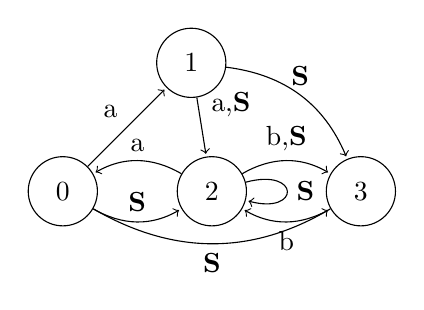
\begin{tikzpicture}[shorten >=1pt,auto]
        \node[state] (q_0)                      {$0$};
        \node[state] (q_1) [above right=of q_0] {$1$};
        \node[state] (q_2) [right=of q_0]       {$2$};
        \node[state] (q_3) [right=of q_2]       {$3$};
          \path[->]
            (q_0) edge  node {a} (q_1)
            (q_1) edge  node {a,\textbf{S}} (q_2)
            (q_2) edge[bend right, above]  node {a} (q_0)
            (q_2) edge[loop right]  node {\textbf{S}} (q_2)
            (q_1) edge[bend left, above]  node {\textbf{S}} (q_3)
            (q_0) edge[bend right, above]  node {\textbf{S}} (q_2)
            (q_2) edge[bend left, above]  node {b,\textbf{S}} (q_3)
            (q_0) edge[bend right, below]  node {\textbf{S}} (q_3)
            (q_3) edge[bend left, below]  node {b} (q_2);
    \end{tikzpicture}
    \caption{The result graph $\mathcal{G}$}
    \label{example:result}
    \end{center}
    \end{subfigure}
    \caption{The input and result graphs for example}
    \label{example:input_and_result}

\end{figure}

Adjacency matrices $M_1$ and $M_2$ for automata $R$ and graph $\mathcal{G}$ respectively are initialized as follows:
    $$
    M_1 =
    \begin{pmatrix}
    . & \{a\} & . & .     \\
    . & . & \{S\} & \{b\} \\
    . & . & . & \{b\}     \\
    . & . & . & .
    \end{pmatrix}
    ,~~~~~
    M_2^0 =
    \begin{pmatrix}
    . & \{a\} & . & .     \\
    . & . & \{a\} & .     \\
    \{a\} & . & . & \{b\} \\
    . & . & \{b\} & .
    \end{pmatrix}.
    $$

After the initialization in lines \textbf{2--4}, the algorithm handles $\varepsilon$-case.
Because the machine $R$ does not have $\varepsilon$-transitions and $\varepsilon$-word is not included in the language, lines \textbf{5--7} of the algorithm do not affect the input data.

Then the algorithm enters the while loop and iterates while matrix $M_2$ is changing.
We provide both the values of the matrices $M_3$, $C_3$ at each algorithm step as well as how the matrix $M_2$ is updated.
The current loop iteration number is provided in the superscript for each matrix.
The first iteration is indexed as 1.

During the first iteration the Kronecker product $M_3^1 = M_1 \otimes M_2^0$ and transitive closure $C_3^1$ are the following:

%\begin{figure}
    {\tiny
    \renewcommand{\arraystretch}{0.6}
    %\centering
    $$
    M_3^1 =
    \left(
    \begin{array}{c c c c | c c c c | c c c c | c c c c }
    . & . & . & .  &  . & 1 & . & .  &  . & . & . & .  &  . & . & . & .   \\
    . & . & . & .  &  . & . & 1 & .  &  . & . & . & .  &  . & . & . & .   \\
    . & . & . & .  &  1 & . & . & .  &  . & . & . & .  &  . & . & . & .   \\
    . & . & . & .  &  . & . & . & .  &  . & . & . & .  &  . & . & . & .   \\
    \hline
    . & . & . & .  &  . & . & . & .  &  . & . & . & .  &  . & . & . & .   \\
    . & . & . & .  &  . & . & . & .  &  . & . & . & .  &  . & . & . & .   \\
    . & . & . & .  &  . & . & . & .  &  . & . & . & .  &  . & . & . & 1   \\
    . & . & . & .  &  . & . & . & .  &  . & . & . & .  &  . & . & 1 & .   \\
    \hline
    . & . & . & .  &  . & . & . & .  &  . & . & . & .  &  . & . & . & .   \\
    . & . & . & .  &  . & . & . & .  &  . & . & . & .  &  . & . & . & .   \\
    . & . & . & .  &  . & . & . & .  &  . & . & . & .  &  . & . & . & 1   \\
    . & . & . & .  &  . & . & . & .  &  . & . & . & .  &  . & . & 1 & . \\
    \hline
    . & . & . & .  &  . & . & . & .  &  . & . & . & .  &  . & . & . & .   \\
    . & . & . & .  &  . & . & . & .  &  . & . & . & .  &  . & . & . & .   \\
    . & . & . & .  &  . & . & . & .  &  . & . & . & .  &  . & . & . & .   \\
    . & . & . & .  &  . & . & . & .  &  . & . & . & .  &  . & . & . & .
    \end{array}
    \right)
    ,~~~~~~
    C_3^1 =
    \left(
    \begin{array}{c c c c | c c c c | c c c c | c c c c }
    . & . & . & .  &  . & 1 & . & .  &  . & . & . & .  &  . & . & . & . \\
    . & . & . & .  &  . & . & 1 & .  &  . & . & . & .  &  . & . & . & \cellcolor{lightgray}\textbf{1} \\
    . & . & . & .  &  1 & . & . & .  &  . & . & . & .  &  . & . & . & . \\
    . & . & . & .  &  . & . & . & .  &  . & . & . & .  &  . & . & . & . \\
    \hline
    . & . & . & .  &  . & . & . & .  &  . & . & . & .  &  . & . & . & . \\
    . & . & . & .  &  . & . & . & .  &  . & . & . & .  &  . & . & . & . \\
    . & . & . & .  &  . & . & . & .  &  . & . & . & .  &  . & . & . & 1 \\
    . & . & . & .  &  . & . & . & .  &  . & . & . & .  &  . & . & 1 & . \\
    \hline
    . & . & . & .  &  . & . & . & .  &  . & . & . & .  &  . & . & . & . \\
    . & . & . & .  &  . & . & . & .  &  . & . & . & .  &  . & . & . & . \\
    . & . & . & .  &  . & . & . & .  &  . & . & . & .  &  . & . & . & 1 \\
    . & . & . & .  &  . & . & . & .  &  . & . & . & .  &  . & . & 1 & . \\
    \hline
    . & . & . & .  &  . & . & . & .  &  . & . & . & .  &  . & . & . & . \\
    . & . & . & .  &  . & . & . & .  &  . & . & . & .  &  . & . & . & . \\
    . & . & . & .  &  . & . & . & .  &  . & . & . & .  &  . & . & . & . \\
    . & . & . & .  &  . & . & . & .  &  . & . & . & .  &  . & . & . & .
    \end{array}
    \right).
    $$
    }
    %\caption{The first iteration tensor product and transitive closure evaluation for example query}
    %\label{example:iteration1eval}
%\end{figure}

%Note here that the dimension $n$ of the matrix $M_3$ equals 16, and this value is constant in time of the algorithm execution.

After the transitive closure evaluation $C_3^1[1,15]$ contains a non-zero value.
It means that the vertex with index $15$ is accessible from the vertex with index $1$ in the graph, represented by the adjacency matrix $M_3^1$.

Then the lines \textbf{14--18} are executed: the algorithm adds non-terminals to the graph matrix $M_2^1$.
Because this step is additive we are only interested in the newly appeared values in the matrix $C_3^1$, such as value $C_3^1[1,15]$, for which we get the following:
\begin{itemize}
    \item Indices of the automata vertices $s = 0$ and $f = 3$, because value $C_3^1[1,15]$ is located in the upper right matrix block $(0,3)$.
    \item Indices of the graph vertices $x = 1$ and $y = 3$ are evaluated as the
    value $C_3^1[1,15]$ indices relatively to its block $(0,3)$.
    \item The function $getNonterminals()$ returns $\{S\}$ since this is the only non-terminal which could be derived in path from vertex $0$ to $3$ in the box $S$.
\end{itemize}

Thus we can conclude that the vertex with $id = 3$ is reachable from the vertex with $id = 1$ by the path derivable from $S$.
As a result, $S$ is added to the $M_2^1[1,3]$.
The updated matrix and graph after the first iteration are presented in figure~\ref{example:iteration1res}.

\begin{figure}[h]
    \begin{subfigure}[]{0.5\textwidth}
    \centering
    $$
    M_2^1 =
    \begin{pmatrix}
    . & \{a\} & . & .     \\
    . & . & \{a\} & \{\textbf{S}\} \\
    \{a\} & . & . & \{b\} \\
    . & . & \{b\} & .
    \end{pmatrix}
    $$
    \end{subfigure}
    \begin{subfigure}[]{0.4\textwidth}
    \centering
    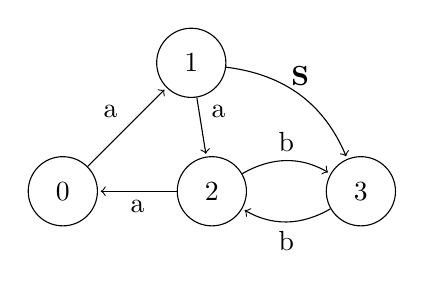
\begin{tikzpicture}[shorten >=1pt,auto]
           \node[state] (q_0)                      {$0$};
           \node[state] (q_1) [above right=of q_0] {$1$};
           \node[state] (q_2) [right=of q_0]       {$2$};
           \node[state] (q_3) [right=of q_2]       {$3$};
            \path[->]
            (q_0) edge  node {a} (q_1)
            (q_1) edge  node {a} (q_2)
            (q_1) edge[bend left, above]  node {\textbf{S}} (q_3)
            (q_2) edge  node {a} (q_0)
            (q_2) edge[bend left, above]  node {b} (q_3)
            (q_3) edge[bend left, below]  node {b} (q_2);
    \end{tikzpicture}
    \end{subfigure}
    \caption{Example: the updated matrix $M_2^1$ and graph $\mathcal{G}$ after first loop iteration}
    \label{example:iteration1res}
\end{figure}


For the second iteration matrices $M_3^2$ and $C_3^2$ are evaluated as follows:
{
\tiny
    \renewcommand{\arraystretch}{0.6}
    \centering
    $$
    M_3^2 =
    \left(
    \begin{array}{c c c c | c c c c | c c c c | c c c c }
    . & . & . & .  &  . & 1 & . & .  &  . & . & . & .  &  . & . & . & .   \\
    . & . & . & .  &  . & . & 1 & .  &  . & . & . & .  &  . & . & . & .   \\
    . & . & . & .  &  1 & . & . & .  &  . & . & . & .  &  . & . & . & .   \\
    . & . & . & .  &  . & . & . & .  &  . & . & . & .  &  . & . & . & .   \\
    \hline
    . & . & . & .  &  . & . & . & .  &  . & . & . & .           &  . & . & . & .   \\
    . & . & . & .  &  . & . & . & .  &  . & . & . & \cellcolor{lightgray}\textbf{1}  &  . & . & . & .   \\
    . & . & . & .  &  . & . & . & .  &  . & . & . & .           &  . & . & . & 1 \\
    . & . & . & .  &  . & . & . & .  &  . & . & . & .           &  . & . & 1 & . \\
    \hline
    . & . & . & .  &  . & . & . & .  &  . & . & . & .  &  . & . & . & .   \\
    . & . & . & .  &  . & . & . & .  &  . & . & . & .  &  . & . & . & .   \\
    . & . & . & .  &  . & . & . & .  &  . & . & . & .  &  . & . & . & 1 \\
    . & . & . & .  &  . & . & . & .  &  . & . & . & .  &  . & . & 1 & . \\
    \hline
    . & . & . & .  &  . & . & . & .  &  . & . & . & .  &  . & . & . & .   \\
    . & . & . & .  &  . & . & . & .  &  . & . & . & .  &  . & . & . & .   \\
    . & . & . & .  &  . & . & . & .  &  . & . & . & .  &  . & . & . & .   \\
    . & . & . & .  &  . & . & . & .  &  . & . & . & .  &  . & . & . & .
    \end{array}
    \right),
    C_3^2 =
    \left(
    \begin{array}{c c c c | c c c c | c c c c | c c c c }
    . & . & . & .  &  . & 1 & . & .  &  . & . & . & \cellcolor{lightgray}\textbf{1}  &  . & . & \cellcolor{lightgray}\textbf{1} & . \\
    . & . & . & .  &  . & . & 1 & .  &  . & . & . & .  &  . & . & . & 1 \\
    . & . & . & .  &  1 & . & . & .  &  . & . & . & .  &  . & . & . & . \\
    . & . & . & .  &  . & . & . & .  &  . & . & . & .  &  . & . & . & . \\
    \hline
    . & . & . & .  &  . & . & . & .  &  . & . & . & .  &  . & . & . & . \\
    . & . & . & .  &  . & . & . & .  &  . & . & . & 1  &  . & . & \cellcolor{lightgray}\textbf{1} & . \\
    . & . & . & .  &  . & . & . & .  &  . & . & . & .  &  . & . & . & 1 \\
    . & . & . & .  &  . & . & . & .  &  . & . & . & .  &  . & . & 1 & . \\
    \hline
    . & . & . & .  &  . & . & . & .  &  . & . & . & .  &  . & . & . & . \\
    . & . & . & .  &  . & . & . & .  &  . & . & . & .  &  . & . & . & . \\
    . & . & . & .  &  . & . & . & .  &  . & . & . & .  &  . & . & . & 1 \\
    . & . & . & .  &  . & . & . & .  &  . & . & . & .  &  . & . & 1 & . \\
    \hline
    . & . & . & .  &  . & . & . & .  &  . & . & . & .  &  . & . & . & . \\
    . & . & . & .  &  . & . & . & .  &  . & . & . & .  &  . & . & . & . \\
    . & . & . & .  &  . & . & . & .  &  . & . & . & .  &  . & . & . & . \\
    . & . & . & .  &  . & . & . & .  &  . & . & . & .  &  . & . & . & .
    \end{array}
    \right).
    $$
}
%listed in Figure~\ref{example:iteration2eval}.
New non-zero values in the matrix $C_3^2$ have appeared during this iteration in cells with indices $[0,11]$, $[0,14]$ and $[5,14]$.
Because only the cell value with index $[0,14]$ corresponds to the automata path with not empty non-terminal set $\{S\}$ its data affects the adjacency matrix $M_2$.
The updated matrix and graph $\mathcal{G}$ are shown in Figure~\ref{example:iteration2res}.

%\begin{figure}
%    \caption{The second iteration tensor product and transitive closure evaluation for example query}
%    \label{example:iteration2eval}
%\end{figure}

\begin{figure}
    \begin{subfigure}[]{0.5\textwidth}
    \centering
    $$
    M_2^2 =
    \begin{pmatrix}
    .     & \{a\} & \{\textbf{S}\} & .     \\
    .     & .     & \{a\} & \{S\} \\
    \{a\} & .     & .     & \{b\} \\
    .     & .     & \{b\} & .
    \end{pmatrix}
    $$
    \end{subfigure}
    \begin{subfigure}[]{0.4\textwidth}
    \centering
    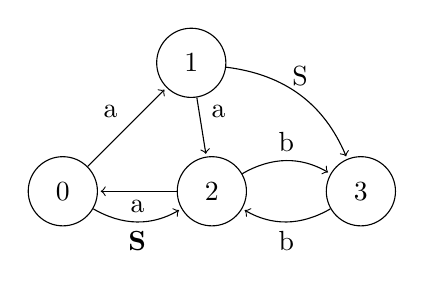
\begin{tikzpicture}[shorten >=1pt,auto]
           \node[state] (q_0)                      {$0$};
           \node[state] (q_1) [above right=of q_0] {$1$};
           \node[state] (q_2) [right=of q_0]       {$2$};
           \node[state] (q_3) [right=of q_2]       {$3$};
            \path[->]
            (q_0) edge  node {a} (q_1)
            (q_1) edge  node {a} (q_2)
            (q_1) edge[bend left, above]  node {S} (q_3)
            (q_2) edge  node {a} (q_0)
            (q_0) edge[bend right, below]  node {\textbf{S}} (q_2)
            (q_2) edge[bend left, above]  node {b} (q_3)
            (q_3) edge[bend left, below]  node {b} (q_2);
    \end{tikzpicture}
    \end{subfigure}
    \caption{Example: the updated matrix $M_2^2$ and graph $\mathcal{G}$ after second loop iteration}
    \label{example:iteration2res}
\end{figure}

The remaining matrices $C_3$ and $M_2$ for the algorithm's main loop execution are listed in the Figure~\ref{example:iteration3to6eval} and Figure~\ref{example:iteration3to6res} correspondingly.
The evaluated matrices $M_3$ are not included because its computation is straightforward.
The last loop iteration is $7$.
Although the matrix $M_2^6$ is updated with the new non-terminal $S$ for the cell $[2,2]$ after the transitive closure evaluation, the new values are not added to the matrix $M_2$.
Therefore matrix $M_2$ has stopped changing and the algorithm has finished.
The graph $\mathcal{G}$ with the new edges is presented in the Figure~\ref{example:result}.

\begin{figure}[ht]
    \tiny
    \renewcommand{\arraystretch}{0.6}
    \centering
    $$
    C_3^3 =
    \left(
    \begin{array}{c c c c | c c c c | c c c c | c c c c }
    . & . & . & .  &  . & 1 & . & .  &  . & . & . & 1  &  . & . & 1 & . \\
    . & . & . & .  &  . & . & 1 & .  &  . & . & . & .  &  . & . & . & 1 \\
    . & . & . & .  &  1 & . & . & .  &  . & . & \cellcolor{lightgray}\textbf{1} & .  &  . & . & . & \cellcolor{lightgray}\textbf{1} \\
    . & . & . & .  &  . & . & . & .  &  . & . & . & .  &  . & . & . & . \\
    \hline
    . & . & . & .  &  . & . & . & .  &  . & . & 1 & .  &  . & . & . & \cellcolor{lightgray}\textbf{1} \\
    . & . & . & .  &  . & . & . & .  &  . & . & . & 1  &  . & . & 1 & . \\
    . & . & . & .  &  . & . & . & .  &  . & . & . & .  &  . & . & . & 1 \\
    . & . & . & .  &  . & . & . & .  &  . & . & . & .  &  . & . & 1 & . \\
    \hline
    . & . & . & .  &  . & . & . & .  &  . & . & . & .  &  . & . & . & . \\
    . & . & . & .  &  . & . & . & .  &  . & . & . & .  &  . & . & . & . \\
    . & . & . & .  &  . & . & . & .  &  . & . & . & .  &  . & . & . & 1 \\
    . & . & . & .  &  . & . & . & .  &  . & . & . & .  &  . & . & 1 & . \\
    \hline
    . & . & . & .  &  . & . & . & .  &  . & . & . & .  &  . & . & . & . \\
    . & . & . & .  &  . & . & . & .  &  . & . & . & .  &  . & . & . & . \\
    . & . & . & .  &  . & . & . & .  &  . & . & . & .  &  . & . & . & . \\
    . & . & . & .  &  . & . & . & .  &  . & . & . & .  &  . & . & . & .
    \end{array}
    \right)
    C_3^4 =
    \left(
    \begin{array}{c c c c | c c c c | c c c c | c c c c }
    . & . & . & .  &  . & 1 & . & .  &  . & . & . & 1  &  . & . & 1 & . \\
    . & . & . & .  &  . & . & 1 & .  &  . & . & . & \cellcolor{lightgray}\textbf{1}  &  . & . & \cellcolor{lightgray}\textbf{1} & 1 \\
    . & . & . & .  &  1 & . & . & .  &  . & . & 1 & .  &  . & . & . & 1 \\
    . & . & . & .  &  . & . & . & .  &  . & . & . & .  &  . & . & . & . \\
    \hline
    . & . & . & .  &  . & . & . & .  &  . & . & 1 & .  &  . & . & . & 1 \\
    . & . & . & .  &  . & . & . & .  &  . & . & . & 1  &  . & . & 1 & . \\
    . & . & . & .  &  . & . & . & .  &  . & . & . & 1  &  . & . & \cellcolor{lightgray}\textbf{1} & 1 \\
    . & . & . & .  &  . & . & . & .  &  . & . & . & .  &  . & . & 1 & . \\
    \hline
    . & . & . & .  &  . & . & . & .  &  . & . & . & .  &  . & . & . & . \\
    . & . & . & .  &  . & . & . & .  &  . & . & . & .  &  . & . & . & . \\
    . & . & . & .  &  . & . & . & .  &  . & . & . & .  &  . & . & . & 1 \\
    . & . & . & .  &  . & . & . & .  &  . & . & . & .  &  . & . & 1 & . \\
    \hline
    . & . & . & .  &  . & . & . & .  &  . & . & . & .  &  . & . & . & . \\
    . & . & . & .  &  . & . & . & .  &  . & . & . & .  &  . & . & . & . \\
    . & . & . & .  &  . & . & . & .  &  . & . & . & .  &  . & . & . & . \\
    . & . & . & .  &  . & . & . & .  &  . & . & . & .  &  . & . & . & .
    \end{array}
    \right)
    $$
    $$
    C_3^5 =
    \left(
    \begin{array}{c c c c | c c c c | c c c c | c c c c }
    . & . & . & .  &  . & 1 & . & .  &  . & . & \cellcolor{lightgray}\textbf{1} & 1  &  . & . & 1 & \cellcolor{lightgray}\textbf{1} \\
    . & . & . & .  &  . & . & 1 & .  &  . & . & . & 1  &  . & . & 1 & 1 \\
    . & . & . & .  &  1 & . & . & .  &  . & . & 1 & .  &  . & . & . & 1 \\
    . & . & . & .  &  . & . & . & .  &  . & . & . & .  &  . & . & . & . \\
    \hline
    . & . & . & .  &  . & . & . & .  &  . & . & 1 & .  &  . & . & . & 1 \\
    . & . & . & .  &  . & . & . & .  &  . & . & 1 & 1  &  . & . & 1 & \cellcolor{lightgray}\textbf{1} \\
    . & . & . & .  &  . & . & . & .  &  . & . & . & 1  &  . & . & 1 & 1 \\
    . & . & . & .  &  . & . & . & .  &  . & . & . & .  &  . & . & 1 & . \\
    \hline
    . & . & . & .  &  . & . & . & .  &  . & . & . & .  &  . & . & . & . \\
    . & . & . & .  &  . & . & . & .  &  . & . & . & .  &  . & . & . & . \\
    . & . & . & .  &  . & . & . & .  &  . & . & . & .  &  . & . & . & 1 \\
    . & . & . & .  &  . & . & . & .  &  . & . & . & .  &  . & . & 1 & . \\
    \hline
    . & . & . & .  &  . & . & . & .  &  . & . & . & .  &  . & . & . & . \\
    . & . & . & .  &  . & . & . & .  &  . & . & . & .  &  . & . & . & . \\
    . & . & . & .  &  . & . & . & .  &  . & . & . & .  &  . & . & . & . \\
    . & . & . & .  &  . & . & . & .  &  . & . & . & .  &  . & . & . & .
    \end{array}
    \right)
    C_3^6 =
    \left(
    \begin{array}{c c c c | c c c c | c c c c | c c c c }
    . & . & . & .  &  . & 1 & . & .  &  . & . & 1 & 1  &  . & . & 1 & 1 \\
    . & . & . & .  &  . & . & 1 & .  &  . & . & . & 1  &  . & . & 1 & 1 \\
    . & . & . & .  &  1 & . & . & .  &  . & . & 1 & \cellcolor{lightgray}\textbf{1}  &  . & . & \cellcolor{lightgray}\textbf{1} & 1 \\
    . & . & . & .  &  . & . & . & .  &  . & . & . & .  &  . & . & . & . \\
    \hline
    . & . & . & .  &  . & . & . & .  &  . & . & 1 & 1  &  . & . & \cellcolor{lightgray}\textbf{1} & 1 \\
    . & . & . & .  &  . & . & . & .  &  . & . & 1 & 1  &  . & . & 1 & 1 \\
    . & . & . & .  &  . & . & . & .  &  . & . & . & 1  &  . & . & 1 & 1 \\
    . & . & . & .  &  . & . & . & .  &  . & . & . & .  &  . & . & 1 & . \\
    \hline
    . & . & . & .  &  . & . & . & .  &  . & . & . & .  &  . & . & . & . \\
    . & . & . & .  &  . & . & . & .  &  . & . & . & .  &  . & . & . & . \\
    . & . & . & .  &  . & . & . & .  &  . & . & . & .  &  . & . & . & 1 \\
    . & . & . & .  &  . & . & . & .  &  . & . & . & .  &  . & . & 1 & . \\
    \hline
    . & . & . & .  &  . & . & . & .  &  . & . & . & .  &  . & . & . & . \\
    . & . & . & .  &  . & . & . & .  &  . & . & . & .  &  . & . & . & . \\
    . & . & . & .  &  . & . & . & .  &  . & . & . & .  &  . & . & . & . \\
    . & . & . & .  &  . & . & . & .  &  . & . & . & .  &  . & . & . & .
    \end{array}
    \right)
    $$
    \caption{Transitive closure for loop iterations $3-6$ for example query}
    \label{example:iteration3to6eval}
\end{figure}

\begin{figure}[ht]
\tiny
    \centering
    $$
    M_2^3 =
    \begin{pmatrix}
    .     & \{a\} & \{S\} & .       \\
    .     & .     & \{a\} & \{S\}   \\
    \{a\} & .     & .     & \{b,\textbf{S}\} \\
    .     & .     & \{b\} & .
    \end{pmatrix}
    M_2^4 =
    \begin{pmatrix}
    .     & \{a\} & \{S\}   & .       \\
    .     & .     & \{a,\textbf{S}\} & \{S\}   \\
    \{a\} & .     & .       & \{b,S\} \\
    .     & .     & \{b\}   & .
    \end{pmatrix}
    $$
    $$
    M_2^5 =
    \begin{pmatrix}
    .     & \{a\} & \{S\}   & \{\textbf{S}\}   \\
    .     & .     & \{a,S\} & \{S\}   \\
    \{a\} & .     & .       & \{b,S\} \\
    .     & .     & \{b\}   & .
    \end{pmatrix}
    M_2^6 =
    \begin{pmatrix}
    .     & \{a\} & \{S\}   & \{S\}   \\
    .     & .     & \{a,S\} & \{S\}   \\
    \{a\} & .     & \{\textbf{S}\}   & \{b,S\} \\
    .     & .     & \{b\}   & .
    \end{pmatrix}
    $$
    \caption{The updated matrix $M_2$ for loop iterations $3-6$ for example query}
    \label{example:iteration3to6res}
\end{figure}
\section{Evaluation}

The goal of this evaluation is to investigate the applicability of the proposed algorithm to both regular and context-free path querying.
We measured the execution time of the index creation which solves the reachability problem for both kinds of queries.
The execution time for CFPQ was compared with the Azimov's algorithm for CFPQ reachability.
We also investigated the practical applicability of paths extraction algorithm to both regular and context-free path queries.

For evaluation, we used a PC with Ubuntu 18.04 installed.
It has Intel core i7-6700 CPU, 3.4GHz, and DDR4 64Gb RAM.
We only measure the execution time of the algorithms themselves, thus we assume an input graph is loaded into RAM in the form of its adjacency matrix in the sparse format.
Note, that the time needed to load an input graph into the RAM is excluded from the time measurements.

\subsection{RPQ Evaluation}

To investigate the applicability of the proposed algorithm for regular path querying we gathered a dataset which consists of both real-world and synthetically generated graphs.
We generated the queries from the most popular RPQ templates.

\subsubsection{Dataset}

We gathered several graphs which represent real-world data from different areas and are frequently used for evaluation of the graph querying algorithms.
Namely, the dataset consists of three parts.
The first part is the set of LUBM graphs\footnote{Lehigh University Benchmark (LUBM) web page: \url{http://swat.cse.lehigh.edu/projects/lubm/}. Access date: 07.07.2020.}~\citep{10.1016/j.websem.2005.06.005} which have different numbers of vertices.
The second one is the set of graphs from Uniprot database\footnote{Universal Protein Resource (UniProt) web page: \url{https://www.uniprot.org/}. All files used can be downloaded via the link: \url{ftp://ftp.uniprot.org/pub/databases/uniprot/current_release/rdf/}. Access date: 07.07.2020.}: \textit{proteomes}, \textit{taxonomy} and \textit{uniprotkb}.
The~last part consists of the RDF files \textit{mappingbased\_properties} from DBpedia\footnote{DBpedia project web site: \url{https://wiki.dbpedia.org/}. Access date: 07.07.2020.} and \textit{geospecies}\footnote{The Geospecies RDF: \url{https://old.datahub.io/dataset/geospecies}. Access date: 07.07.2020.}.
A brief description of the graphs in the dataset is presented in Table~\ref{tbl:graphs_for_rpq}.

\begin{table}
    \centering
\caption{Graphs for RPQ evaluation}
\label{tbl:graphs_for_rpq}
{

\rowcolors{2}{black!2}{black!10}
\begin{tabular}{|l|c|c|}
\hline
Graph & \#V & \#E  \\
\hline
\hline
LUBM1k  & 120 926 & 484 646 \\
LUBM3.5k  & 358 434 & 144 9711 \\
LUBM5.9k  & 596 760 & 2 416 513 \\
LUBM1M   & 1 188 340 & 4 820 728 \\
LUBM1.7M & 1 780 956 & 7 228 358 \\
LUBM2.3M & 2 308 385 & 9 369 511 \\
\hline
Uniprotkb & 6 442 630 & 24 465 430 \\
Proteomes & 4 834 262 & 12 366 973 \\
Taxonomy & 5 728 398 & 14 922 125 \\
\hline
Geospecies & 450 609 & 2 201 532 \\
Mappingbased\_properties & 8 332 233 & 25 346 359 \\
\hline
\end{tabular}
}
\end{table}


Queries for evaluation were generated from the templates for the most popular RPQs, specifically the queries presented in Table 2 in~\cite{Pacaci2020RegularPQ} and in Table 5 in~\cite{Wang2019}.
These query templates are presented in Table~\ref{tbl:queries_templates}.
We generate 10 queries for each template and each graph.
The most frequent relations from the given graph were used as symbols in the query template\footnote{Used generator is available as part of CFPQ\_data project: \url{https://github.com/JetBrains-Research/CFPQ_Data/blob/master/tools/gen_RPQ/gen.py}. Access data: 07.07.2020.}.
We used the same set of queries for all LUBM graphs to investigate scalability of the proposed algorithm.

\begin{table}
    \centering
\caption{Queries templates for RPQ evaluation}
\label{tbl:queries_templates}
{\small
\renewcommand{\arraystretch}{1.2}
\rowcolors{2}{black!2}{black!10}
\begin{tabular}{|c|c||c|c|}
\hline

Name & Query & Name & Query \\
\hline
\hline
$Q_1$   & $a^*$                               & $Q_9^5$    & $(a \mid b \mid c \mid d \mid e)^+$                     \\
$Q_2$   & $a\cdot b^*$                        & $Q_{10}^2$ & $(a \mid b) \cdot c^*$                                  \\
$Q_3$   & $a \cdot b^* \cdot c^*$             & $Q_{10}^3$ & $(a \mid b \mid c)  \cdot d^*$                          \\
$Q_4^2$ & $(a \mid b)^*$                      & $Q_{10}^4$ & $(a \mid b \mid c \mid d)  \cdot e^*$                   \\
$Q_4^3$ & $(a \mid b \mid c)^*$               & $Q_{10}^5$ & $(a \mid b \mid c \mid d \mid e)  \cdot f^*$            \\
$Q_4^4$ & $(a \mid b \mid c \mid d)^*$        & $Q_{10}^2$ & $a \cdot b$                                             \\
$Q_4^5$ & $(a \mid b \mid c \mid d \mid e)^*$ & $Q_{11}^3$ & $a \cdot b \cdot c$                                     \\
$Q_5$   & $a \cdot b^* \cdot c$               & $Q_{11}^4$ & $a \cdot b \cdot c \cdot d$                             \\
$Q_6$   & $a^* \cdot b^*$                     & $Q_{11}^5$ & $a \cdot b \cdot c \cdot d \cdot f$                     \\
$Q_7$   & $a \cdot b \cdot c^*$               & $Q_{12}$   & $(a \cdot b)^+ \mid  (c \cdot d)^+$                     \\
$Q_8$   & $a? \cdot b^*$                      & $Q_{13}$   & $(a \cdot(b \cdot c)^*)^+ \mid  (d \cdot f)^+$          \\
$Q_9^2$ & $(a \mid b)^+$                      & $Q_{14}$   & $(a \cdot b \cdot (c \cdot d)^*)^+  \cdot (e \mid f)^*$ \\
$Q_9^3$ & $(a \mid b \mid c)^+$               & $Q_{15}$   & $(a \mid b)^+ \cdot (c \mid d)^+$                       \\
$Q_9^4$ & $(a \mid b \mid c \mid d)^+$        & $Q_{16}$   & $a \cdot b \cdot (c \mid d \mid e)$                     \\
\hline
\end{tabular}
}
\end{table}


\subsubsection{Results}

We averaged the execution time of index creation over 5 runs for each query.
Index creation time for LUBM graphs set is presented in Figure~\ref{fig:lubm_all_qs}.
We can see that evaluation time depends on the query: there are queries which evaluate in less than 1 second even for the largest graphs ($Q_2$, $Q_5$, $Q_{11}^2$, $Q_{11}^3$), while the worst time is 6.26 seconds ($Q_{14}$).
The execution time of our algorithm is comparable with the recent results for the same graphs and queries implemented on a distributed system over 10 nodes~\citep{Wang2019}, while we use only one node.
We conclude that our algorithm demonstrates reasonable performance to be applied to the real-world data analysis.
%\cho{Note that the accurate comparison of different approaches may be a promising direction of future research.}

\begin{figure}
    \centering
   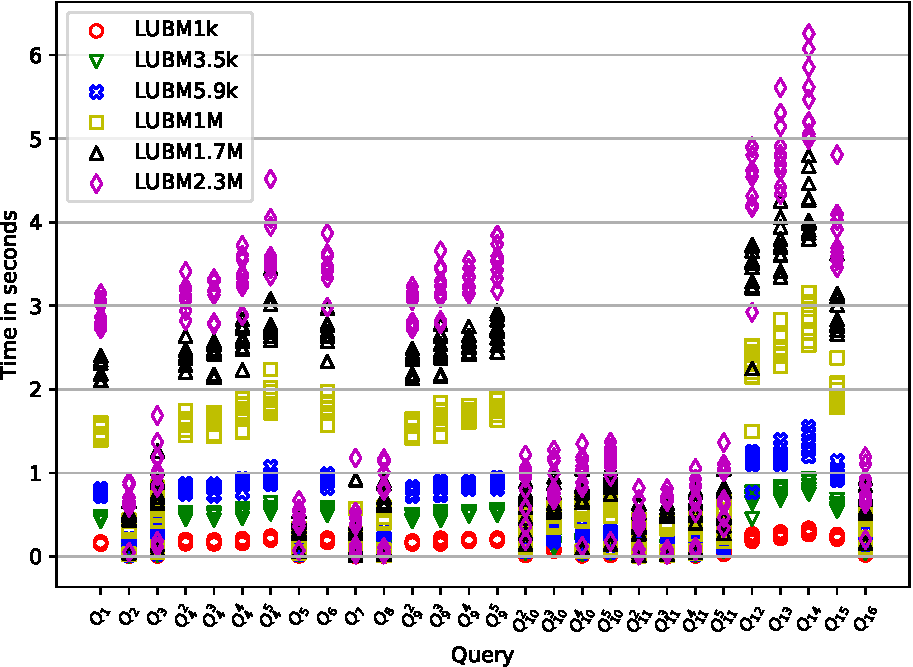
\includegraphics[width=0.6\textwidth]{data/LUBM_all.pdf}
   \caption{Index creation time for LUBM graphs}
   \label{fig:lubm_all_qs}
\end{figure}

Index creation time for each query on the real-world graphs is presented in Figure~\ref{fig:other_all_qs}.
We can see that querying small graphs requires more time than querying bigger graphs in some cases.
For example, conseder $Q_{10}^4$: querying the \textit{geospecies} graph (450k vertices) in some cases requires more time than querying of \textit{mappingbased\_properties} (8.3M vertices) and \textit{taxonomy} (5.7M vertices).
We conclude that the evaluation time depends on the inner structure of a graph.
On the other hand, \textit{taxonomy} querying in many cases requires significantly more time than for other graphs, while \textit{taxonomy} is not the biggest graph.
Finally, in most cases query execution lasts less than 10 seconds, even for bigger graphs, and no query requires more than 52.17 seconds.

\begin{figure}
    \centering
   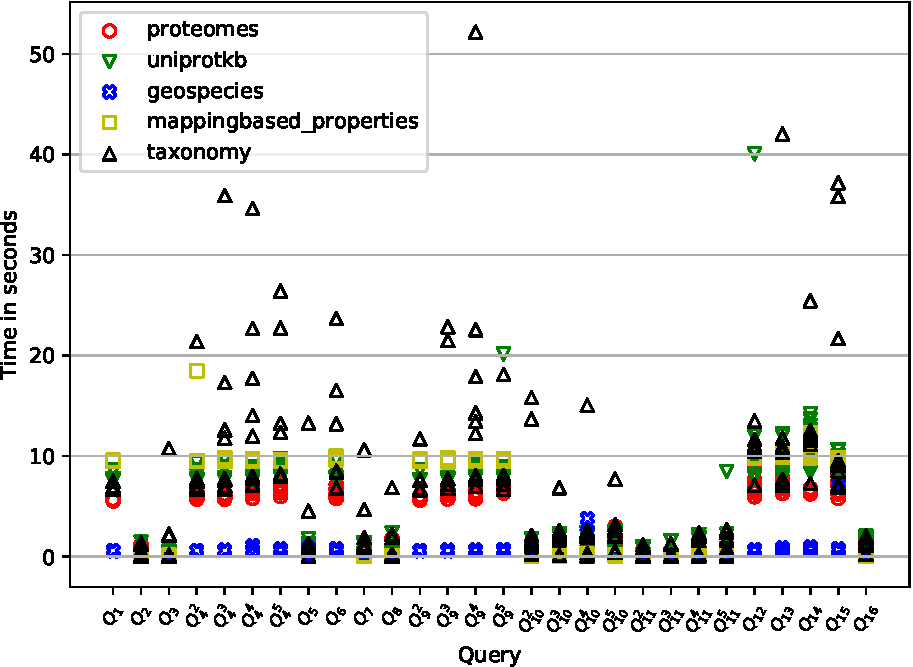
\includegraphics[width=0.6\textwidth]{data/other_all.pdf}
   \caption{Index creation time for real-world RDFs}
   \label{fig:other_all_qs}
\end{figure}

%We evaluate path extraction for queries which result in possibly long paths.
%Long paths usually require many iterations of transitive closure evaluation, thus we used the number of the iterations as a criterion to select the inputs for the evaluation.
%For each selected graph and query we measure paths extraction time for each reachable pair.
%Since the index can be reused from the previous step, we omit the time necessary to create the index.
%We limit by 10 the number of paths to extract.

%In Figures~\ref{fig:geo_tensors_rpq} and~\ref{fig:dbpedia_tensors_rpq} we show the time needed to extract a path of a specific length when only one path was extracted.
%The main observation is that time is linear on the path length, even if a generic path extraction procedure is used.

%\begin{figure}
%     \begin{subfigure}[b]{0.45\textwidth}
%         \centering
%         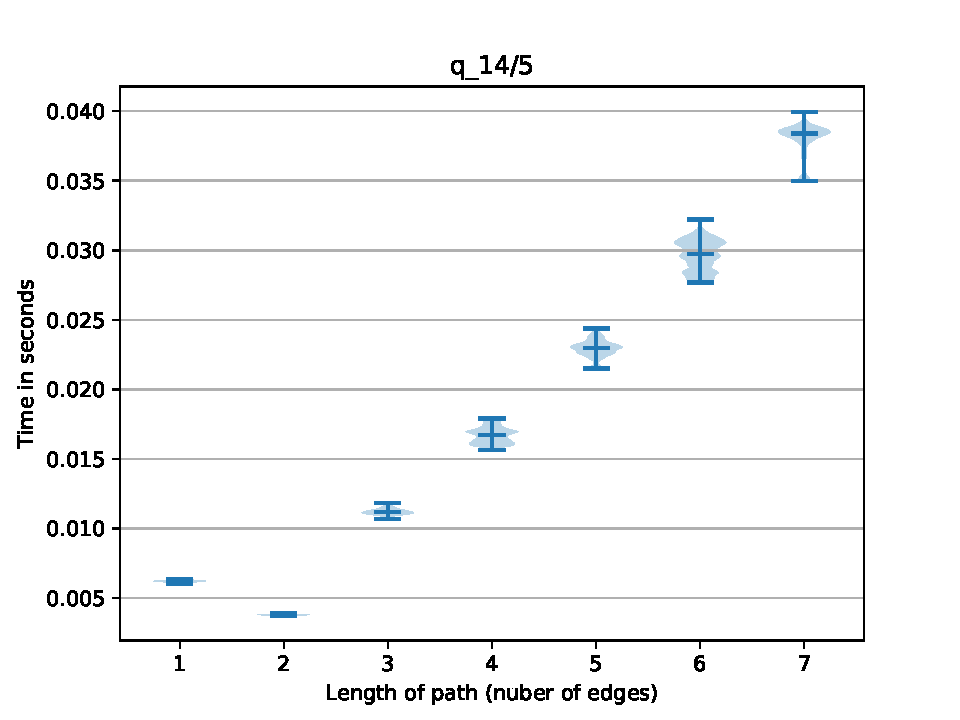
\includegraphics[width=\textwidth]{../paper/data/geo_rpq_single_path/q_14_5.pdf}
%         \caption{\footnotesize \textit{geospecies}, $Q_{14}$}
%         \label{fig:geo_tensors_rpq}
%     \end{subfigure}
%     ~\begin{subfigure}[b]{0.45\textwidth}
%         \centering
%         \includegraphics[width=\textwidth]{../paper/data/CF/Tensor_path/dbpedia_path_tensor.pdf}
%         \caption{\footnotesize \textit{mappingbased\_properties}, $Q_{4}^5$}
%         \label{fig:dbpedia_tensors_rpq}
%     \end{subfigure}\\
%     \begin{subfigure}[b]{0.45\textwidth}
%         \centering
%         \includegraphics[width=\textwidth]{../paper/data/CF/Matrix_CF/geo_path_matrix.pdf}
%         \caption{\footnotesize \textit{geospecies}, \textit{Geo}}
%         \label{fig:geo_matrix_cfpq}
%     \end{subfigure}
%     ~\begin{subfigure}[b]{0.45\textwidth}
%         \centering
%         \includegraphics[width=\textwidth]{../paper/data/CF/Tensor_path/geo_path_tensor.pdf}
%         \caption{\footnotesize \textit{geospecies}, \textit{Geo}}
%         \label{fig:geo_tensors_cfpq}
%     \end{subfigure}\\
%   \caption{Single path extraction for specific graph and query for our solution (\subref{fig:geo_tensors_rpq}, \%subref{fig:dbpedia_tensors_rpq}, \subref{fig:geo_tensors_cfpq}), and Azimov's (\subref{fig:geo_matrix_cfpq})}
%\end{figure}

\subsection{CFPQ Evaluation}

We evaluate the applicability of the proposed algorithm to CFPQ processing over real-world graphs on a number of classic cases and compare them with the Azimov's algorithm.
Currently only a single path version of Azimov's algorithm exists, and we use its implementation using PyGraphBLAS. Note that it is not trivial to compare our results with the state-of-the-art results provided by~\cite{10.1145/3398682.3399163} (Azimov's algorithm) because our algorithm computes significantly more information. While the state-of-the-art solution computes only reachability facts or a single-path semantics, our algorithm computes data necessary to restore all possible paths.

\subsubsection{Dataset}

We use CFPQ\_Data\footnote{CFPQ\_Data is a dataset for CFPQ evaluation which contains both synthetic and real-world data and queries \url{https://github.com/JetBrains-Research/CFPQ\_Data}. Access date: 07.07.2020.} dataset for evaluation.
Namely, we use relatively big RDF files and respective same-generation queries $G_1$~(Eq.~\ref{eqn:g_1}) and $G_2$~(Eq.~\ref{eqn:g_2}) which are used in other works for CFPQ evaluation.
We also use the $Geo$~(Eq.~\ref{eqn:geo}) query provided by~\cite{Kuijpers:2019:ESC:3335783.3335791} for \textit{geospecies} RDF.
Note that we use $\overline{x}$ notation in queries to denote the inverse of $x$ relation and the respective edge.
\begin{align}
\begin{split}
\label{eqn:g_1}
S \to & \overline{\textit{subClassOf}} \ \ S \ \textit{subClasOf} \mid \overline{\textit{type}} \ \ S \ \textit{type}\\   & \mid \overline{\textit{subClassOf}} \ \ \textit{subClasOf} \mid \overline{\textit{type}} \ \textit{type}
\end{split}
\end{align}
\begin{align}
\begin{split}
\label{eqn:g_2}
S \to \overline{\textit{subClassOf}} \ \ S \ \textit{subClasOf} \mid \textit{subClassOf}
\end{split}
\end{align}
\begin{align}
\begin{split}
\label{eqn:geo}
S \to & \textit{broaderTransitive} \ \  S \ \overline{\textit{broaderTransitive}} \\
      & \mid \textit{broaderTransitive} \ \  \overline{\textit{broaderTransitive}}
\end{split}
\end{align}
\begin{align}
\begin{split}
\label{eqn:ma}
S & \to \overline{d} \ V \ d \\
V & \to ((S?) \overline{a})^* (S?) (a (S?))^*
\end{split}
\end{align}

Additionally we evaluate our algorithm on memory aliases analysis problem: a well-known problem which can be reduced to CFPQ~\citep{Zheng:2008:DAA:1328897.1328464}.
To do it, we use some graphs built for different parts of Linux OS kernel (\textit{arch}, \textit{crypto}, \textit{drivers}, \textit{fs}) and the query $MA$~(Eq.~\ref{eqn:ma})~\citep{10.1145/3093336.3037744}.
The detailed data about all the graphs used is presented in Table~\ref{tbl:graphs_for_cfpq}.

{\setlength{\tabcolsep}{0.3em}
\begin{table}
    \centering
{
\caption{Graphs for CFPQ evaluation: \textit{bt} is broaderTransitive, \textit{sco} is subCalssOf}
\label{tbl:graphs_for_cfpq}
\scriptsize
\rowcolors{2}{black!2}{black!10}
\begin{tabular}{|l|c|c|c|c|c|c|c|}
\hline
Graph          & \#V       & \#E        & \#sco & \#type &\#bt & \#a  & \#d \\
\hline
\hline
eclass\_514en  & 239 111    & 523 727    & 90 512    & 72 517    &        ---        & ---  & --- \\
enzyme         & 48 815     & 109 695    & 8 163     & 14 989    &        ---        & ---  & --- \\
geospecies     & 450 609    & 2 201 532  & 0         & 89 062    &        20 867     & ---  & --- \\
go             & 272 770    & 534 311    & 90 512    & 58 483    &        ---        & ---  & --- \\
go-hierarchy   & 45 007     & 980 218    & 490 109   & 0         &        ---        & ---  & --- \\
taxonomy       & 5 728 398  & 14 922 125 & 2 112 637 & 2 508 635 &        ---        & ---  & --- \\
\hline
arch           & 3 448 422  & 5 940 484  &      ---     &  ---   &        ---        & 671 295 & 2 298 947 \\
crypto         & 3 464 970  & 5 976 774  &      ---     &  ---   &        ---        & 678 408 & 2 309 979 \\
drivers        & 4 273 803  & 7 415 538  &      ---     &  ---   &        ---        & 858 568 & 2 849 201 \\
fs             & 4 177 416  & 7 218 746  &      ---     &  ---   &        ---        & 824 430 & 2 784 943 \\
\hline
\end{tabular}
}
\end{table}
}
\subsubsection{Results}

We averaged the index creation time over 5 runs for both single-path Azimov's algorithm (\textbf{Mtx}) and the proposed algorithm (\textbf{Tns}) (see Table~\ref{tbl:CFPQ_index}).

{\setlength{\tabcolsep}{0.2em}
  \begin{table}
    \centering
    \caption{CFPQ evaluation results, time is measured in seconds}
    \label{tbl:CFPQ_index}
    \rowcolors{4}{black!2}{black!10}
    \small
    \begin{tabular}{| l | c | c | c | c | c | c | c | c |}
      \hline

      \multirow{2}{*}{Name}  & \multicolumn{2}{c|}{$G_1$} & \multicolumn{2}{c|}{$G_2$} & \multicolumn{2}{c|}{\textit{Geo}} & \multicolumn{2}{c|}{\textit{MA}}\\
      \cline{2-9}
                      & Tns    & Mtx    & Tns  & Mtx  & Tns   & Mtx   & Tns     & Mtx \\
      \hline
      \hline
      eclass\_514en   & 0.24   & 0.27   & 0.25 & 0.26 & ---   & ---   & ---     & ---\\
      enzyme          & 0.03   & 0.04   & 0.02 & 0.01 & ---   & ---   & ---     & ---\\
      geospecies      & 0.08   & 0.06   & $0^{*}$ & 0.01 & 26.12 & 16.58 & ---     & ---\\
      go-hierarchy    & 0.16   & 1.43   & 0.23 & 0.86 & ---   & ---   & ---     & ---\\
      go              & 1.56   & 1.74   & 1.21 & 1.14 & ---   & ---   & ---     & ---\\
      pathways        & 0.01   & 0.01   & 0.01 & 0.01 & ---   & ---   & ---     & ---\\
      taxonomy        & 4.81   & 2.71   & 3.75 & 1.56 & ---   & ---   & ---     & ---\\
      \hline
      arch            & ---    & ---    & ---  & ---  & ---   & ---   & 262.45  & 195.51  \\
      crypto          & ---    & ---    & ---  & ---  & ---   & ---   & 267.52  & 195.54  \\
      drivers         & ---    & ---    & ---  & ---  & ---   & ---   & 1309.57 & 1050.78 \\
      fs              & ---    & ---    & ---  & ---  & ---   & ---   & 470.49  & 370.73  \\
      \hline
    \end{tabular}
  \end{table}
}

Best to our knowledge, the proposed algorithm is the first algorithm that provides information about all paths of interest (Azimov's algorithm computes information about only one path).
The direct comparison with other solutions is impossible, and we just estimate the running time of our algorithm for a small number of cases.
Namely, we extract all paths with length not greater than 20 edges between all pairs of vertices from indeces created for graphs \textit{go} and \textit{eclass\_514en} and query $G_1$.
Paths extraction for one pair of vertices requires 2.64 seconds averaged over all pairs for \textit{go} graph. The~maximal time is 4699 seconds and 217737 paths were extracted during this time. The average number of paths between two vertices is 184.
For \textit{eclass\_514en} paths extraction for one pair of vertices requires 1.27 seconds averaged over all pairs. The~maximal time is 8.04 seconds and only one path is extracted during this time. The average number of paths between two vertices is 3.
We can see that paths can be extracted in a reasonable time, but a detailed analysis of paths extraction algorithm performance depends on graphs structure.

%Comparison of paths extraction is presented in Figures~\ref{fig:geo_matrix_cfpq} and~\ref{fig:geo_tensors_cfpq}.
%While both methods demonstrate linear time on the length of the extracted path, our generic solution is more than 1000 times slower than Azimov's single path extraction procedure.
%We conclude that current generic all-path extraction procedure is not optimal for single path extraction.

\subsection{Conclusion}

We conclude that the proposed algorithm is applicable to real-world data processing: the algorithm allows one to solve both the reachability problem and to extract paths of interest in a reasonable time even using naive implementation.
While index creation time (reachability query evaluation) is comparable with other existing solutions, paths extraction procedure should be improved in the future. However, the state-of-the-art solution computes only reachability facts or a single-path semantics, whereas our algorithm computes data necessary to restore all possible paths (all-paths semantics).
Finally, a detailed comparison of the proposed solution with other algorithms for CFPQ and RPQ is required.

To summarize the overall evaluation, the proposed algorithm is applicable to both RPQ and CFPQ over real-world graphs.
Thus, the proposed solution is a promising unified algorithm for both RPQ and CFPQ evaluation.

\section{Conclusion}

Conclusion, current state, results.

Future work. Library extension up to full GraphBLAS API implementation.

LaGraph on F\# .NET.

Evaluation. Comparison with other implementations on different devices.
Manual implementation versus translation.  

Another direction of future work is Brahma.FSharp improvements. 
First of all, it is necessary to support discriminated unions to make it possible to express custom semirings such as \texttt{Min-Plus}, as presented in listing~\ref{lst_example}. 

Also, it is necessary to add high-level abstractions for asynchronous programming, and for multi-GPU programming.
Such mechanisms can be naturally expressed in F\# with native primitives for asynchronous programming.

fusion and other optimizations.

%
% ---- Bibliography ----
%
% BibTeX users should specify bibliography style 'splncs04'.
% References will then be sorted and formatted in the correct style.
%
 \bibliographystyle{splncs04}
 \bibliography{tensor_product_cfpq}
\end{document}
